% =============================================================================
% HTR-Pipeline: Overall Concept / Workflow Diagram
% -----------------------------------------------------------------------------
% Register-Augmented Vision Transformer for Explainable Handwritten Text
% Recognition (HTR), with dual outputs for recognition accuracy (CTC) and
% attention-based explainability feeding downstream tasks (e.g. writer ID).
%
% Compile standalone:   pdflatex htr_pipeline_diagram.tex
% Include in a report:  1) compile to PDF, then 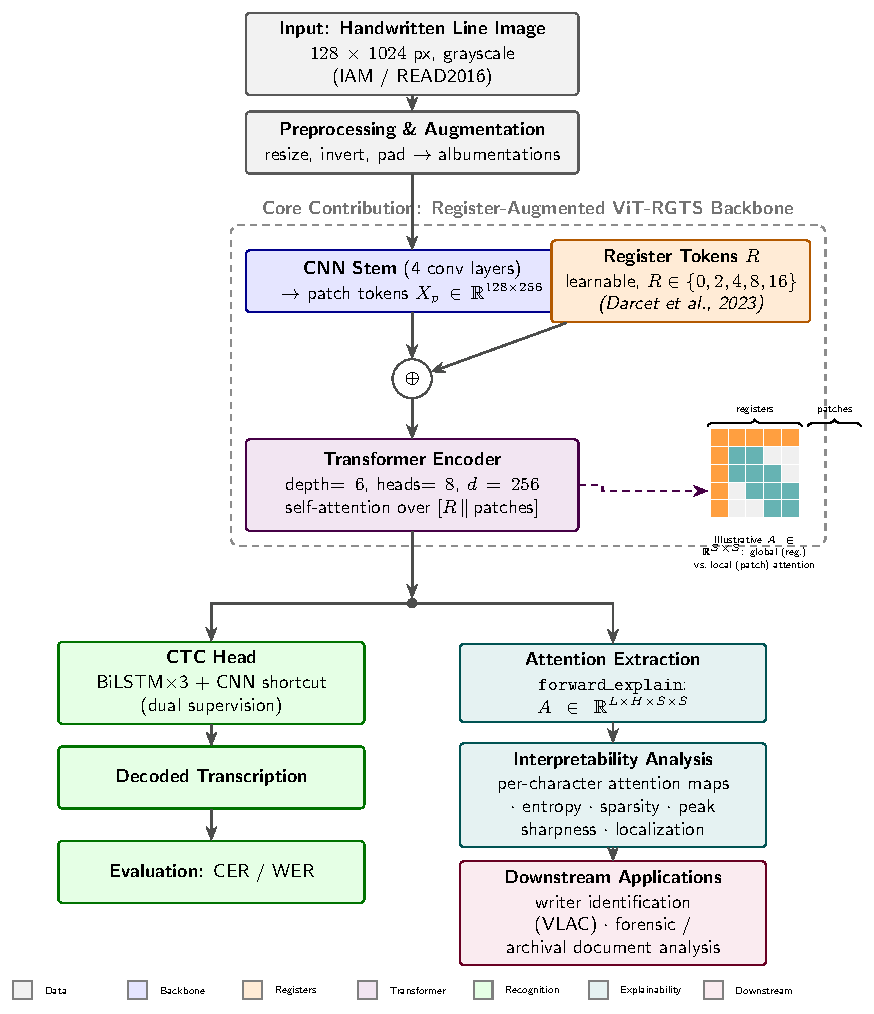
\includegraphics{htr_pipeline_diagram}
%                       2) or copy the tikzpicture body into a \begin{figure} env
%                          of a document that loads the same tikz libraries.
% =============================================================================
\documentclass[tikz,border=6pt]{standalone}
\usepackage{amsmath,amssymb}
\usetikzlibrary{arrows.meta, positioning, shapes.geometric, fit, backgrounds, calc, decorations.pathreplacing}

\begin{document}
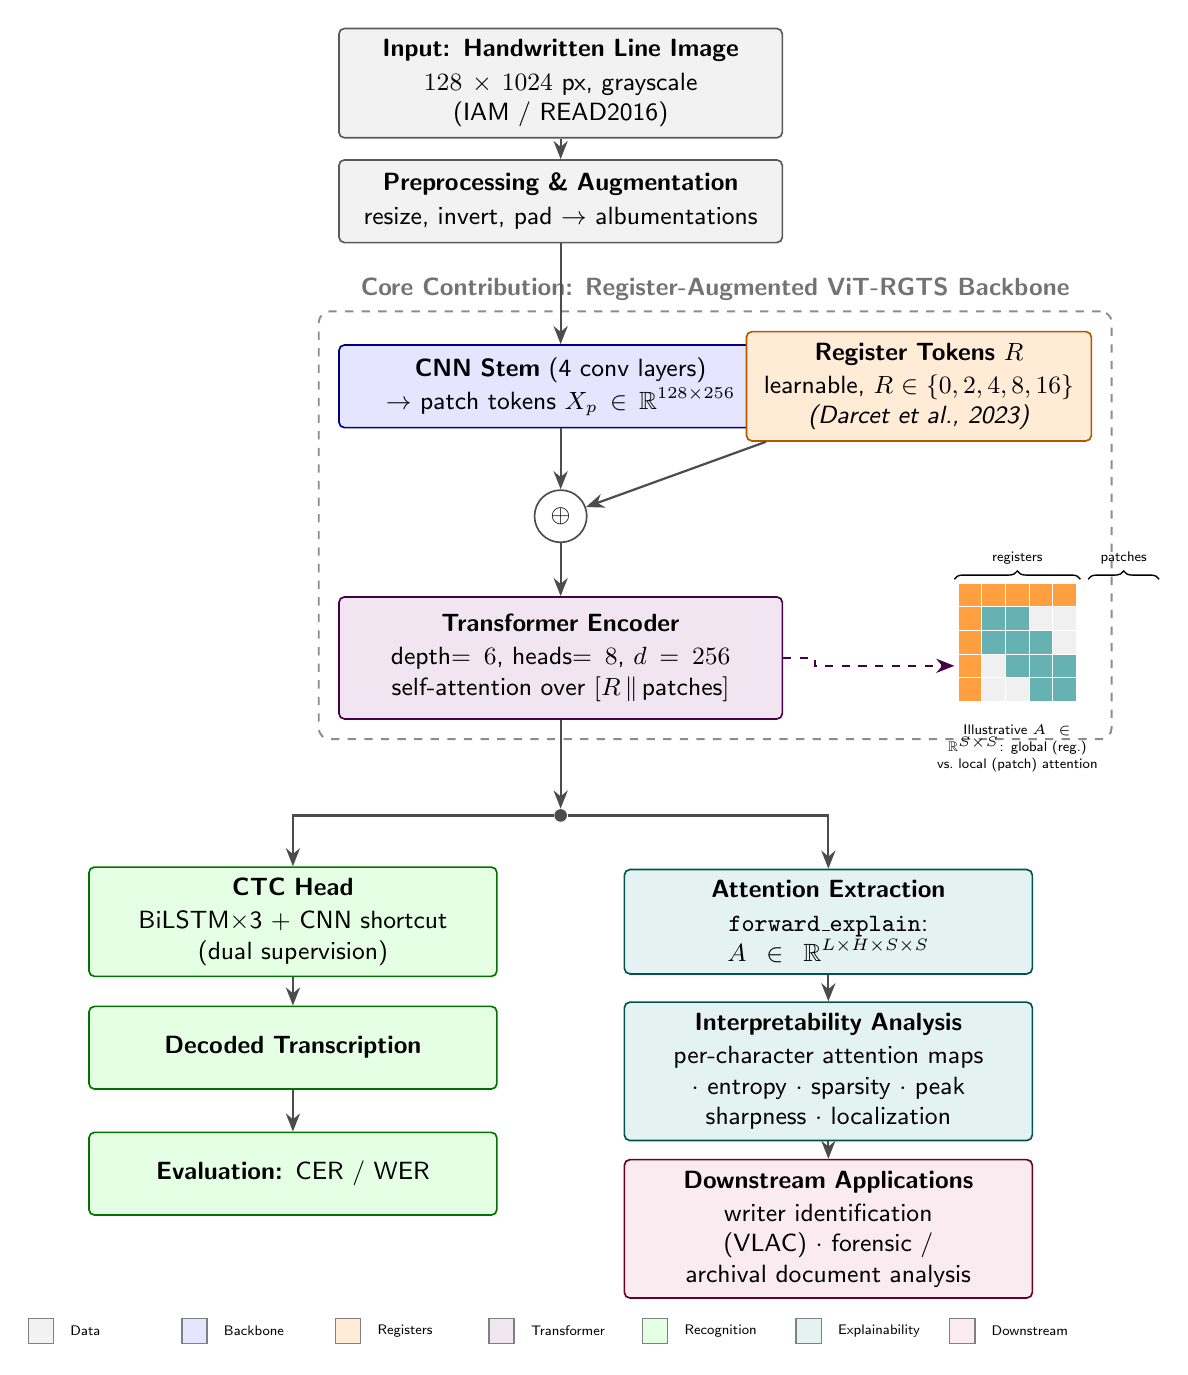
\begin{tikzpicture}[
  font=\sffamily,
  every node/.style={align=center},
  arr/.style={-{Stealth[length=2.3mm, width=1.8mm]}, thick, draw=black!70},
  node distance=8mm and 10mm,
  box/.style={rectangle, rounded corners=2pt, draw=black!65, line width=0.6pt,
              minimum height=1.05cm, text width=5.35cm, inner sep=4pt, font=\sffamily\small},
  data/.style   ={box, fill=black!5},
  cnn/.style    ={box, fill=blue!10, draw=blue!55!black},
  reg/.style    ={box, text width=4.1cm, fill=orange!16, draw=orange!70!black},
  trans/.style  ={box, minimum height=1.55cm, fill=violet!10, draw=violet!55!black},
  ctc/.style    ={box, text width=4.9cm, fill=green!10, draw=green!45!black},
  attn/.style   ={box, text width=4.9cm, fill=teal!10, draw=teal!65!black},
  down/.style   ={box, text width=4.9cm, fill=purple!8, draw=purple!55!black},
  merge/.style  ={circle, draw=black!70, line width=0.6pt, fill=white, minimum size=6mm, font=\small},
  junction/.style={circle, fill=black!70, minimum size=1.6mm, inner sep=0pt},
]

% ---------------------------------------------------------------- main spine
\node[data]  (input)      at (0,12.4)  {\textbf{Input: Handwritten Line Image}\\[1pt] $128\times1024$ px, grayscale (IAM~/~READ2016)};
\node[data]  (prep)       at (0,10.9)  {\textbf{Preprocessing \& Augmentation}\\[1pt] resize, invert, pad $\rightarrow$ albumentations};
\node[cnn]   (stem)       at (0,8.55)  {\textbf{CNN Stem} (4 conv layers)\\[1pt] $\rightarrow$ patch tokens $X_p\in\mathbb{R}^{128\times256}$};

\node[reg]   (regs)       at (4.55,8.55) {\textbf{Register Tokens} $R$\\[1pt] learnable, $R\in\{0,2,4,8,16\}$\\ \emph{(Darcet et al., 2023)}};

\node[merge] (concat)     at (0,6.9)   {$\oplus$};
\node[trans] (transf)     at (0,5.1)   {\textbf{Transformer Encoder}\\[1pt] depth$=6$, heads$=8$, $d=256$\\ self-attention over $[R\,\|\,\text{patches}]$};

% ------------------------------------------------- mini illustrative heatmap
\begin{scope}[shift={(5.05,5.75)}]
  \foreach \i in {1,...,5}{
    \foreach \j in {1,...,5}{
      \pgfmathtruncatemacro{\diff}{abs(\i-\j)}
      \ifnum\i=1 \def\ccol{orange!75}
      \else\ifnum\j=1 \def\ccol{orange!75}
      \else\ifnum\diff<2 \def\ccol{teal!60}
      \else \def\ccol{gray!12}
      \fi\fi\fi
      \draw[fill=\ccol, draw=white, line width=0.35pt]
        ({(\j-1)*0.30},{-(\i-1)*0.30}) rectangle ++(0.30,0.30);
    }
  }
  \draw[decorate, decoration={brace, amplitude=3pt}, line width=0.5pt]
        (-0.05,0.35) -- (1.55,0.35) node[midway, above=2pt, font=\tiny\sffamily]{registers};
  \draw[decorate, decoration={brace, amplitude=3pt}, line width=0.5pt]
        (1.65,0.35) -- (1.65+0.9,0.35) node[midway, above=2pt, font=\tiny\sffamily]{patches};
  \node[font=\tiny\sffamily, text width=2.6cm, align=center] at (0.75,-1.8)
        {Illustrative $A\!\in\!\mathbb{R}^{S\times S}$: global (reg.)\\ vs.\ local (patch) attention};
\end{scope}
\draw[arr, dashed, draw=violet!55!black] (transf.east) -- ++(0.4,0) |- (5.05-0.05,5.75-0.75);

% ----------------------------------------------------- core-contribution box
\begin{scope}[on background layer]
  \node[draw=black!45, dashed, line width=0.7pt, rounded corners=4pt,
        fit=(stem)(regs)(concat)(transf), inner sep=7pt, label={[font=\small\sffamily\bfseries, black!55]above:Core Contribution: Register-Augmented ViT-RGTS Backbone}] (backbone) {};
\end{scope}

% -------------------------------------------------------------- arrows spine
\draw[arr] (input) -- (prep);
\draw[arr] (prep)  -- (stem);
\draw[arr] (stem)  -- (concat);
\draw[arr] (regs)  -- (concat);
\draw[arr] (concat)-- (transf);

% ------------------------------------------------------------------ branches
\node[junction] (split) at (0,3.1) {};
\draw[arr] (transf) -- (split);

\node[ctc]  (ctchead) at (-3.4,1.75) {\textbf{CTC Head}\\[1pt] BiLSTM$\times$3 + CNN shortcut\\ (dual supervision)};
\node[ctc]  (text)    at (-3.4,0.15) {\textbf{Decoded Transcription}};
\node[ctc]  (accmetr) at (-3.4,-1.45){\textbf{Evaluation:} CER / WER};

\node[attn] (aextract) at (3.4,1.75) {\textbf{Attention Extraction}\\[1pt] \texttt{forward\_explain}: $A\in\mathbb{R}^{L\times H\times S\times S}$};
\node[attn] (interp)   at (3.4,-0.15) {\textbf{Interpretability Analysis}\\[1pt] per-character attention maps $\cdot$ entropy $\cdot$ sparsity $\cdot$ peak sharpness $\cdot$ localization};
\node[down] (downstream) at (3.4,-2.15){\textbf{Downstream Applications}\\[1pt] writer identification (VLAC) $\cdot$ forensic / archival document analysis};

\draw[arr] (split) -| (ctchead);
\draw[arr] (split) -| (aextract);
\draw[arr] (ctchead) -- (text);
\draw[arr] (text) -- (accmetr);
\draw[arr] (aextract) -- (interp);
\draw[arr] (interp) -- (downstream);

% ---------------------------------------------------------------------- legend
\begin{scope}[shift={(0,-3.45)}]
  \foreach \i/\col/\lbl in {0/black!5/Data, 1/blue!10/Backbone, 2/orange!16/Registers,
                            3/violet!10/Transformer, 4/green!10/Recognition, 5/teal!10/Explainability, 6/purple!8/Downstream} {
    \node[rectangle, draw=black!50, line width=0.5pt, fill=\col, minimum width=3.2mm, minimum height=3.2mm] at (-6.6+1.95*\i,0) {};
    \node[font=\tiny\sffamily, anchor=west] at (-6.6+1.95*\i+0.25,0) {\lbl};
  }
\end{scope}

\end{tikzpicture}
\end{document}
